\section{An operative numeric parameter has a conditional, nonmonotone response}
\label{sec:native-reserve-response}
\subsection{Measure the component without inventing counterfactual worlds}
The planning search leaves the strong reference's allocation program unchanged.
Before interpreting a numerical search over its reserve, we ask a narrower
question: does this existing parameter change the commands on the actual
inputs that its consumer received? We retain R7's complete original inputs
for years 1--4 and execute its exact archived allocation artifact in the same
pinned sandbox image for every integer reserve $r\in\{1,\ldots,60\}$.
Only the already declared input parameter changes. All 240 calls complete;
at $r=21$, all four complete component returns match their original records.
This adds no scientist-model call or native world and does not alter any
optimizer's feedback or the original study's inputs.

Let $x_y^{(21)}$ denote R7's recorded year-$y$ component input under its
original reserve21 trajectory, and let $C_r$ be the unchanged program with
reserve $r$. The measured object is
\[
  \left(C_r(x_1^{(21)}),\ldots,C_r(x_4^{(21)})\right),
  \qquad r\in\{1,\ldots,60\}.
\]
It is \emph{not} a rollout on the future states $x_y^{(r)}$ induced by each
alternative system. Outputs are requested transfer commands, not newly
committed transfers, participation outcomes or loss evaluations. Consequently,
neither adding commands across recorded years nor maximizing transferred
funds would estimate the optimization target.

\begin{figure}[t]
\centering
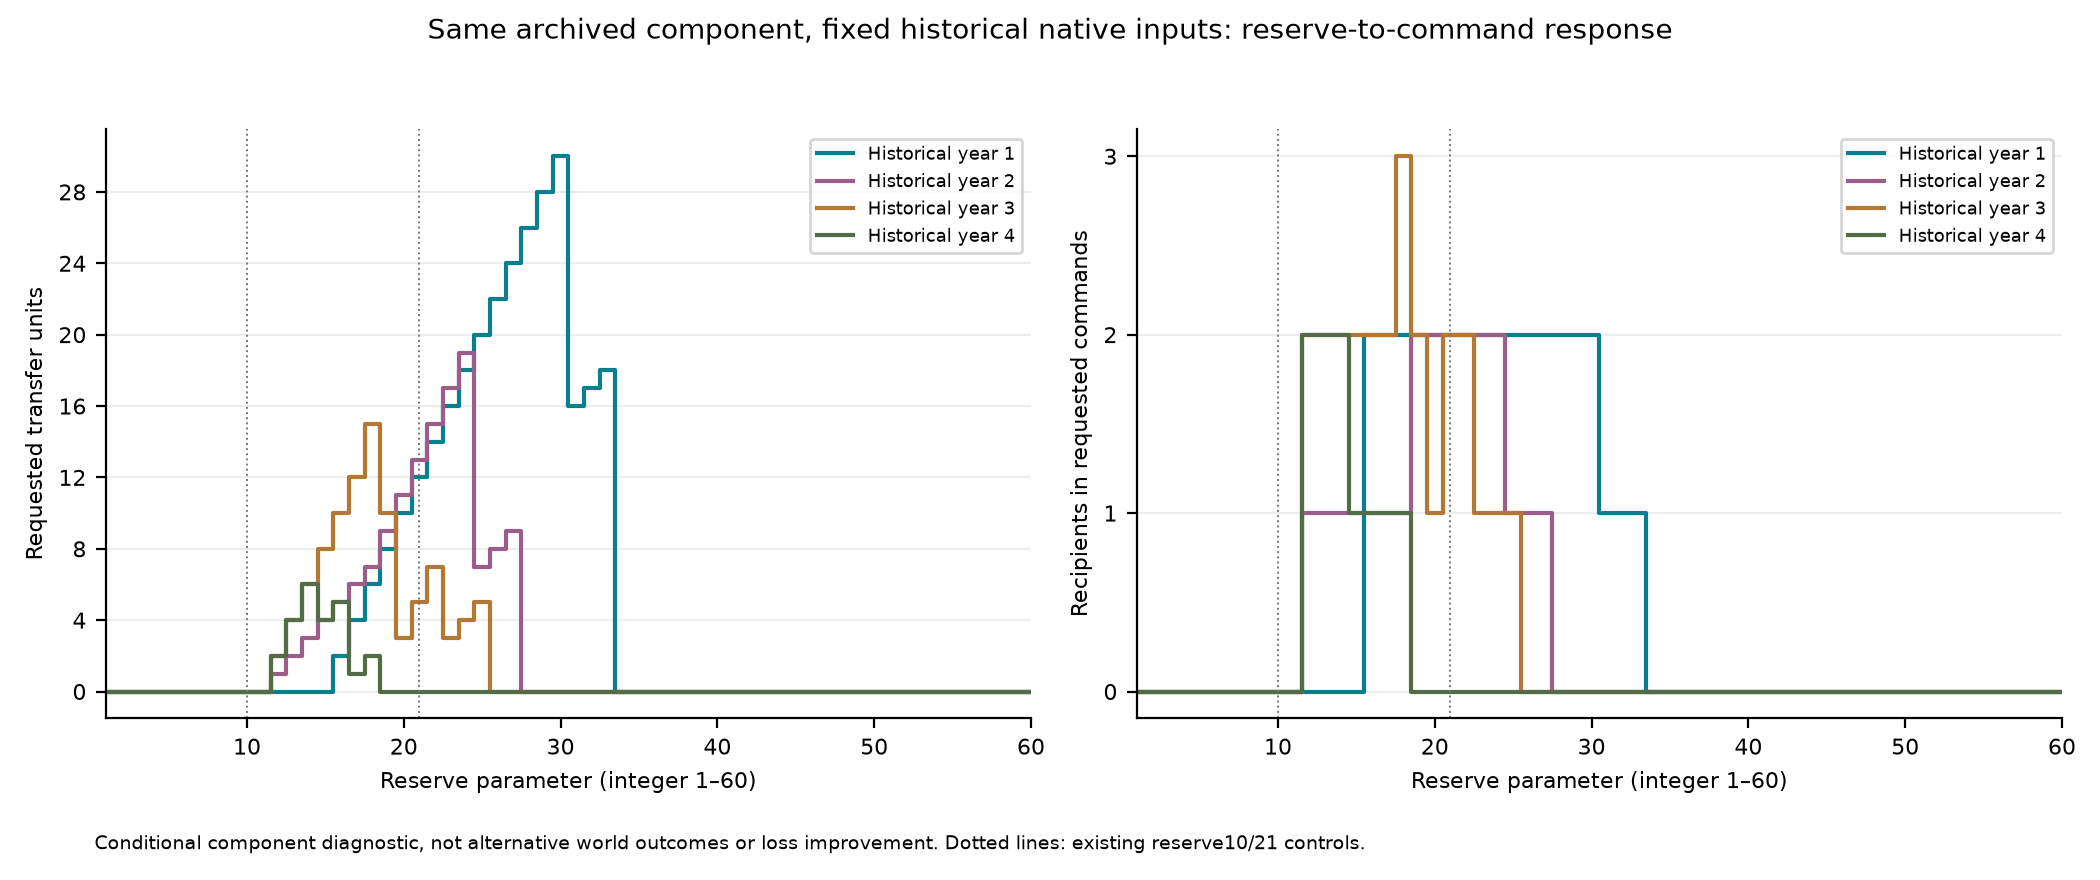
\includegraphics[width=\linewidth]{figures/native-reserve-command-response-v1/reserve-command-response.png}
\caption{The exact archived allocation component on four fixed historical
native input frames, varying only its reserve parameter. Left: requested
transfer units. Right: recipients in those commands. Dotted lines locate the
existing reserve10/21 controls, not selected optima. Curves are conditional
command responses, not alternative scientist-world outcomes or loss paths.}
\label{fig:native-reserve-commands}
\end{figure}

The 60 reserve values produce respectively 19, 17, 15 and 8 distinct exact
transfer-command outputs on the four historical inputs. The joint four-frame
signature has 23 distinct values. The empty command output recurs in disjoint
low and high reserve intervals; we do not merge those intervals into an
unobserved continuous range. Figure~\ref{fig:native-reserve-commands} exposes
why increasing a parameter need not increase even its immediate output. The
program requests complete rescues up to the target reserve, keeps that same
reserve at donors, and skips a recipient if the remaining surplus cannot
cover its whole need. Increasing the target can reduce feasible transfers.
For example, the year3 input gives the following exact command projections.

\begin{table}[t]
\centering\small
\begin{tabular}{lrrrrr}
\toprule
Reserve &18&19&20&21&26\\
\midrule
Requested transfer units &15&10&3&5&0\\
Recipients &3&2&1&2&0\\
\bottomrule
\end{tabular}
\caption{A nonmonotone conditional response on the same original year3 input.
No reserve is ranked by scientific performance in this diagnostic.}
\label{tab:native-reserve-nonmonotone}
\end{table}

This establishes an actual parameter consumer and an irregular exercised
command surface. It does not show that any reserve optimizes T or U. Equal
outputs on these four inputs also do not establish global policy equivalence,
authorize sharing future native jobs, or provide a gradient of full-world loss.

\subsection{Join commands to the one trajectory that actually occurred}
The original reserve21 year3 commands can separately be joined to its real
native resource ledger. The five founders open with balances
$(31,17,11,11,20)$. The component requests 5 units from founder0, with 4 to
founder1 and 1 to founder4; these commands match the realized transfers.
Every founder pays the original annual cost of10, and founder2 receives the
original20-unit grant. Table~\ref{tab:native-reserve-ledger} retains all five
records, including the deactivated researcher. Every accounting residual is
zero and total resources reconcile as $90-50+20=60$. Transfers conserve money
within the group; they do not increase the grant budget or remove costs.

\begin{table}[t]
\centering\small
\begin{tabular}{lrrrrrc}
\toprule
Founder & Opening & Net transfer & Cost & Grant & Closing & Active\\
\midrule
0&31&$-5$&10&0&16&Yes\\
1&17&4&10&0&11&Yes\\
2&11&0&10&20&21&Yes\\
3&11&0&10&0&1&No\\
4&20&1&10&0&11&Yes\\
\midrule
Total&90&0&50&20&60&4/5\\
\bottomrule
\end{tabular}
\caption{All original R7 founder resource records in year3. Founder indices
abbreviate the fixed original institution0000--0004 researcher identities;
the retained ledger preserves their full identifiers. This is the realized
reserve21 trajectory, not outcomes for the other 59 parameter values.}
\label{tab:native-reserve-ledger}
\end{table}

Native attrition occurs after the award: the inherited implementation removes
active authors whose balance is truthy and at most10. Thus a different founder
with pre-award balance1 survives after receiving20, while founder3 at1 exits.
The truthiness check also excludes exactly zero from this particular branch;
we report that simulator convention rather than silently replacing it with
a cleaner threshold. This is an existing world rule, not a fairness floor,
participation objective or promotion veto added by our optimizer.

\paragraph{The next process-design question.}
The timing of observations, transfers, costs and awards can affect eligibility,
actual charged costs and subsequent researcher inputs. Changing that timing
is not the same intervention as changing a reserve within a fixed calendar.
The conditional analysis motivates a separately declared workflow comparison
with unchanged native effect implementations, rather than a larger search
over an allegedly smooth scalar response. It does not predict which workflow
will win, demonstrate autonomous structural invention, or validate an attrition
convention as a real-world science-policy goal.
